% !TEX root = ../thesis.tex

\chapter{Theory and Motivation for Searching for a Dibosonic Resonance}
\label{chap:theory}

\section{Introduction}

The search for new particles has been an ongoing endeavor since the first accelerators came online in the mid-20th century.
% More history here

Today, the Standard Model (SM) remains as the dominant theory describing three of the four known forces, with gravity excluded due to its inability to be renormalized when approached as a quantum field theory.
The theory itself stands as one of the most well-tested models of physics in history, and all elementary particles predicted by the theory have been found, with the Higgs completing the family after being discovered in the summer of 2012.
However, despite the success of this theory, many fundamental questions of physics still remain unanswered.
As previously mentioned, the theory does not include gravity, as it only accounts for the electromagnetic, strong, and weak nuclear forces.
It also does not account for the existence of Dark Matter or Dark Energy, and there are long-standing issues that the theory currently is incapable of addressing, such as the hierarchy problem.
The theory is therefore regarded as incomplete, and efforts to find physics beyond the Standard Model are ongoing.

In this chapter, we briefly explore the main aspects of the Standard Model in section~\ref{sec:SM}, looking at the fundamental particles that it describes and its mathematical foundations.
Later, in section~\ref{sec:VBF}, we describe the theoretical background relevant to the search for a new fundamental particle beyond the Standard Model that this thesis presents.

\section{The Standard Model of Particle Physics}
\label{sec:SM}

The Standard Model is the prevailing theory in particle physics that classifies all known elementary particles, and describes how they interact with each other via the electromagnetic, weak, and strong forces.
The theory came about during the 1960's in order to explain observations made during early collision experiments\footnotemark.
% More history here

\footnotetext{While the theory itself was developed in the 1960's, the term ``Standard Model'' was coined by Pais and Treiman in 1975~\cite{CaoFieldTheory}.} % Citation needed

\subsection{The Elementary Particles}
\label{subsec:particles}

The Standard Model describes the interactions between 17 elementary particles, which are classified by quarks, leptons, gauge bosons, and scalar bosons.
A table of all particles classified by the theory can be seen in Fig.~\ref{fig:standardModel}, labeled with their masses, charges, and spins~\cite{PhysRevD.98.030001}.
Each particle listed has a corresponding antiparticle, which has the same mass as its particle counterpart, but with opposite physical charges.
% More explanation here

\begin{figure}[htbp]
  \centering
  % !TEX root = ../../thesis.tex

\begin{tikzpicture}
  % Quarks
  \draw pic at (0,0) {particle={green!20}{$u$}{up}{$2.2$ MeV/$c^2$}{$2/3$}{$1/2$}};
  \draw pic at (0,-2.2) {particle={green!20}{$d$}{down}{$4.7$ MeV/$c^2$}{$-1/3$}{$1/2$}};
  \draw pic at (2.2,0) {particle={green!20}{$c$}{charm}{$1.28$ GeV/$c^2$}{$2/3$}{$1/2$}};
  \draw pic at (2.2,-2.2) {particle={green!20}{$s$}{strange}{$96$ MeV/$c^2$}{$-1/3$}{$1/2$}};
  \draw pic at (4.4,0) {particle={green!20}{$t$}{top}{$173.1$ GeV/$c^2$}{$2/3$}{$1/2$}};
  \draw pic at (4.4,-2.2) {particle={green!20}{$b$}{bottom}{$4.18$ MeV/$c^2$}{$-1/3$}{$1/2$}};

  % Leptons
  \draw pic at (0,-4.4) {particle={red!20}{$e$}{electron}{$511$ keV/$c^2$}{$-1$}{$1/2$}};
  \draw pic at (0,-6.6) {particle={red!20}{$\nu_e$}{$e$ neutrino}{$<1.0$ eV/$c^2$}{$0$}{$1/2$}};
  \draw pic at (2.2,-4.4) {particle={red!20}{$\mu$}{muon}{$105.66$ MeV/$c^2$}{$-1$}{$1/2$}};
  \draw pic at (2.2,-6.6) {particle={red!20}{$\nu_\mu$}{$\mu$ neutrino}{$<0.17$ eV/$c^2$}{$0$}{$1/2$}};
  \draw pic at (4.4,-4.4) {particle={red!20}{$\tau$}{tau}{$1.7768$ GeV/$c^2$}{$-1$}{$1/2$}};
  \draw pic at (4.4,-6.6) {particle={red!20}{$\nu_\tau$}{$\tau$ neutrino}{$<18.2$ MeV/$c^2$}{$0$}{$1/2$}};

  % Gauge Bosons
  \draw pic at (6.6,0) {particle={blue!20}{$g$}{gluon}{$0$}{$0$}{$1$}};
  \draw pic at (6.6,-2.2) {particle={blue!20}{$\gamma$}{photon}{$0$}{$0$}{$1$}};
  \draw pic at (6.6,-4.4) {particle={blue!20}{$Z$}{$Z$ boson}{$91.19$ GeV/$c^2$}{$0$}{$1$}};
  \draw pic at (6.6,-6.6) {particle={blue!20}{$W$}{$W$ boson}{$80.39$ GeV/$c^2$}{$\pm1$}{$1$}};

  % Higgs Boson
  \draw pic at (8.8,0) {particle={yellow!20}{$H$}{higgs}{$124.97$ GeV/$c^2$}{0}{0}};

  % Labels
  %\draw[fill=black] (0,0) circle (0.5pt);
  \node at (-1,0.8) [anchor=mid east,scale=0.5] {mass};
  \node at (-1,0.5) [anchor=mid east,scale=0.5] {charge};
  \node at (-1,0.2) [anchor=mid east,scale=0.5] {spin};
  \coordinate (d) at (0,-2.2);
  \coordinate (nu) at (0,-6.6);
  \coordinate (w) at (6.6,-6.6);
  \coordinate (h) at (8.8,0);
  \coordinate (u) at (0,0);
  \coordinate (c) at (2.2,0);
  \coordinate (t) at (4.4,0);
  \node at ($(d)+(-1.35,-1)$) [rotate=90,anchor=mid west,text=green!100] {quarks};
  \node at ($(nu)+(-1.35,-1)$) [rotate=90,anchor=mid west,text=red!100] {leptons};
  \node at ($(w)+(1.35,-1)$) [rotate=90,anchor=mid west,text=blue!100] {gauge bosons};
  %\node at ($(h)+(1.35,-1)$) [rotate=90,anchor=mid west,text=yellow!100] {scalar bosons};
  \node at ($(u)+(0,1.35)$) {I};
  \node at ($(c)+(0,1.35)$) {II};
  \node at ($(t)+(0,1.35)$) {III};
\end{tikzpicture}

  \caption{Table of all Standard Model particles grouped by generation and type, labeled with mass, charge, and spin. Particle types are colored green for quarks, red for leptons, blue for gauge bosons, and orange for scalar bosons.}
  \label{fig:standardModel}
\end{figure}

Quarks are spin-1/2 particles that interact via the strong and weak nuclear forces, as well as the electromagnetic force.
The up and down quarks make up the protons and neutrons of everyday matter that we see and interact with.
For example, a proton is made up of two $u$'s and one $d$ ($uud$), while a neutron is made of two $d$'s and one $u$ ($ddu$).
These are just two of the many different combinations of composite particles that can be formed by quarks.
There are two main combinations of quarks to consider: mesons and baryons.
Mesons are composed of one quark and an antiquark, and baryons are composed of three quarks or three antiquarks. % Mention recently observed pentaquark?
For example, pions ($\pi^0$/$\pi^\pm$) were the first mesons to be observed, and can be electrically charged when comprised only of up or down quark-antiquark pairs (i.e., a $\pi^+$ is made from the combination $u\bar{d}$, and a $\pi^-$ is made from $d\bar{u}$), or it can be electrically neutral (i.e., a $\pi^0$ is made from $u\bar{u}$ or $d\bar{d}$). % Citation about observation
On the other hand, protons and neutrons are examples of baryons, as they are each made of three quarks.
% Possibly elaborate more

Leptons, like quarks, are also spin-1/2 particles that can be electrically charged. Unlike quarks, they only interact via the electromagnetic and weak nuclear forces.
The electron is the most familiar lepton, as it is a component of the atoms that are found in everyday interactions.
However, it also has two heavier cousins: the muon and the tau.
Both of these particles have the same charge as the electron, but their masses are much larger.
Finally, leptons also include neutrinos, which are extremely light particles that have no electric charge, and therefore only interact via the weak force.
% Elaborate here

The gauge bosons include the gluon, the photon, and the $W$ and $Z$ bosons.
Each gauge boson is a spin-1 particle that mediates the three fundamental interactions that the Standard Model describes.
Gluons are massless particles that mediate the strong nuclear force, and they only interact with quarks since they are the only particles to carry color charge.
Photons are the most familiar example of the gauge bosons, as we can quite literally see them since light is made of photons.
They are masses particles that mediate the electromagnetic force, and they interact with any particle that is electrically charged.
Finally, the $Z$ and $W$ bosons are massive particles that mediate the weak nuclear force, which is responsible for radioactive decay.
% Elaborate here

The last category of bosons to consider is the scalar bosons, which are spin-0 particles.
This family contains only one member: the Higgs boson.
The Higgs boson is responsible for giving all massive Standard Model particles their masses, with the exception of the neutrinos.
% More on the Higgs mechanism here
% Discovery of the Higgs in 2012~\cite{20121,201230,Chatrchyan_2013}

\subsection{Mathematical Structure of the Standard Model}

\subsection{Beyond the Standard Model}

As previously mentioned, despite the success of the Standard Model in making predictions about three of the four known fundamental forces of nature, there are many observations that it cannot currently explain.
One major outstanding issue is the inability of the Standard Model to deal with the hierarchy problem.
Using three fundamental constants, one may define the Planck mass as
\begin{equation}
  m_P=\sqrt{\frac{\hbar c}{G}}\approx1.22\times10^{19}\unit{MeV/\clight^2},
\end{equation}
where $\hbar$ is the reduced Planck constant, $c$ is the speed of light, and $G$ is Newton's gravitational constant.
This defines an energy scale at which effects due to gravity would become apparent in particle physics experiments~\cite{QFTNutshell}.
However, this energy scale is vastly larger than what can be obtained in contemporary accelerators.
Fig.~\ref{fig:hierarchy} shows the comparison between the Planck scale, the electroweak symmetry breaking scale, and the current center of mass energy $\sqrt{s}$ at the Large Hadron Collider.

Multiple beyond the Standard Model (BSM) mechanisms have been proposed to deal with the hierarchy problem.


\begin{figure}[htbp]
  \centering
  % !TEX root = ../../thesis.tex

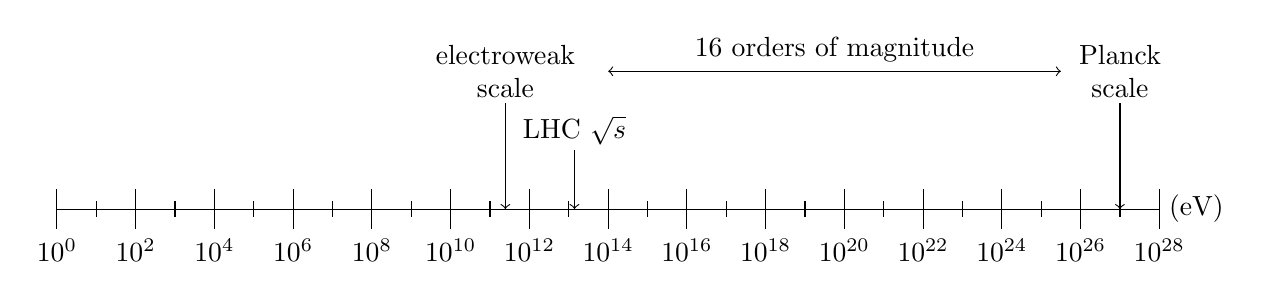
\begin{tikzpicture}
  % Axis
  \draw (0,0) -- (14,0) node[right] {(eV)};
  \draw (0,-0.25) -- (0,0.25);
  \node[below] at (0,-0.25) {$10^0$};
  \foreach \i in {1,...,14}
  {
    % Ticks
    \pgfmathsetmacro{\y}{\i-0.5}
    \draw (\i,-0.25) -- (\i,0.25);
    \draw (\y,-0.1) -- (\y,0.1);

    % Numerical labels
    \pgfmathtruncatemacro{\x}{\i*2}
    \node[below] at (\i,-0.25) {$10^{\x}$};
  }

  % Labels
  \draw[->] (5.695,1.75) node[fill=white,inner sep=2pt,align=center] {electroweak\\scale} -- (5.695,0);
  \draw[->] (6.573,1) node[fill=white,inner sep=2pt] {LHC $\sqrt{s}$} -- (6.573,0);
  \draw[->] (13.5,1.75) node[fill=white,inner sep=2pt,align=center] {Planck\\scale} -- (13.5,0);
  \draw[<->] (7,1.75) -- (12.75,1.75) node[pos=0.5,above] {16 orders of magnitude};
\end{tikzpicture}

  \caption{Comparison between the electroweak scale, LHC center of mass energy $\sqrt{s}$, and Planck scale in eV. The hierarchy problem arises due to the unexplained difference between the Planck scale at which gravitational effects become apparent and the energy scale at which electroweak symmetry breaking occurs, which is 17 orders of magnitude.}
  \label{fig:hierarchy}
\end{figure}

\section{Search for a Heavy Diboson Resonance and Vector Boson Fusion Production Method}
\label{sec:VBF}

In this work, we present results on the search for a new heavy $X$ boson.
% Elaborate more

\subsection{Candidate Bosons}

The search is model independent, and covers the following three possibilities:

\paragraph{Spin-0 Kaluza-Klein Radion}
A neutral scalar boson that appears in Randall-Sundrum (RS) models that can decay to the vector bosons $W$ and $Z$ via $\mathrm{Rad}\to WW$ and $\mathrm{Rad}\to ZZ$~\cite{Goldberger_1999,Goldberger_2000}.

\paragraph{Spin-1 $W'$/$Z'$ Boson}
A heavier version of the spin-1 $W$ and $Z$ bosons that can decay via $W'\to WZ$ and $Z'\to WW$~\cite{Pappadopulo_2014}.

\paragraph{Spin-2 Bulk Graviton}
A spin-2 resonance from a bulk RS model that decays via $G_\mathrm{bulk}\to WW$ or $G_\mathrm{bulk}\to ZZ$~\cite{Fitzpatrick_2007,PhysRevD.76.036006}.

Each possibility for the $X$ boson couples to the massive $V=W,Z$ vector bosons, and each are expected to have masses above 1 TeV.
The decay process is $X\to WV$ with a semi-leptonic final state in which one of the vector bosons is a $W$ that decays leptonically via $W\to\ell\nu$, while the other $V$ boson is either a $W$ or a $Z$ that undergoes $V\to q\bar{q}^{(\prime)}$.
This process was selected due to the fact that one-lepton events are ideal for such an analysis, as the events that are generated provide a clean signal that suppresses background events.
The complete Feynman diagram for the process can be seen in Fig.~\ref{fig:vbfFeynman}.

\subsection{Expected Event Structure}

\begin{figure}[htbp]
  \centering
  % !TEX root = ../../thesis.tex

\begin{tikzpicture}
  \begin{feynman}
    % Vertices
    \coordinate (q1) at (-2.25,1);
    \coordinate (q2) at (0,1);
    \coordinate (q3) at ($(q2)+(25:2.25)$);
    \coordinate (q4) at (-2.25,-1);
    \coordinate (q5) at (0,-1);
    \coordinate (q6) at ($(q5)+(-25:2.25)$);
    \coordinate (v1) at (1.5,0);
    \coordinate (x) at (3.75,0);
    \coordinate (v2) at (5.25,1);
    \coordinate (v3) at (5.25,-1);
    \coordinate (q7) at ($(v2)+(25:1.5)$);
    \coordinate (q8) at ($(v2)+(-25:1.5)$);
    \coordinate (l1) at ($(v3)+(25:1.5)$);
    \coordinate (l2) at ($(v3)+(-25:1.5)$);

    % Lines
    \draw[fermion] (q1) -- (q2);
    \draw[fermion] (q2) -- (q3);
    \draw[fermion] (q4) -- (q5);
    \draw[fermion] (q5) -- (q6);
    \draw[boson] (q2) -- (v1) node[pos=0.65,xshift=-0.5cm] {$V$};
    \draw[boson] (q5) -- (v1) node[pos=0.65,xshift=-0.5cm] {$V$};
    \draw[boson] (v1) -- (x) node[pos=0.5,above] {$X$};
    \draw[boson] (x) -- (v2) node[pos=0.5,xshift=-0.5cm] {$V$};
    \draw[boson] (x) -- (v3) node[pos=0.5,xshift=-0.5cm] {$W$};
    \draw[fermion] (v2) -- (q7);
    \draw[fermion] (q8) -- (v2);
    \draw[fermion] (v3) -- (l1);
    \draw[fermion] (l2) -- (v3);

    % Labels
    \node[anchor=mid,left] (q1n) at (q1) {$q$};
    \node[anchor=mid,left] (q4n) at (q4) {$q$};
    \node[anchor=mid,right] (q3n) at (q3) {$q^{(\prime)}$};
    \node[anchor=mid,right] (q6n) at (q6) {$q^{(\prime)}$};
    \node[anchor=mid,right] (q7n) at (q7) {$q$};
    \node[anchor=mid,right] (q8n) at (q8) {$\bar{q}^{(\prime)}$};
    \node[anchor=mid,right] (l1n) at (l1) {$\ell$};
    \node[anchor=mid,right] (l2n) at (l2) {$\bar{\nu}$};
  \end{feynman}
\end{tikzpicture}

  \caption{Feynman diagram for the production of a generic resonance $X$ via vector boson fusion and decaying to the final state $\ell\nu q\bar{q}'$, with additional forward-facing jets due to the VBF production process. The search for the $X$ boson will involve looking for a final state in which there are jets from the VBF production process present, along with a single merged jet from the $V$ boson, and a lepton $\ell$ with its corresponding neutrino $\nu$ produced from the $W$ decay.}
  \label{fig:vbfFeynman}
\end{figure}

\begin{figure}[htbp]
  \centering
  % !TEX root = ../../thesis.tex
\begin{tikzpicture}
  % Axis
  \draw[->] (-6,0) -- (6,0) node[right] {$z$};

  % Leptons
  \draw[->,thick] (0,0) -- (105:3) node[left] {$\ell$};
  \draw[->,thick] (0,0) -- (75:3) node[right] {$\nu$};

  % Main jet
  \draw[rotate around={180:(0,0)},dotted,thick] (0,2) ellipse (1.3 and 0.4);
  \draw[rotate around={180:(0,0)},dotted,thick] (0,0) -- (56.427:2.3);
  \draw[rotate around={180:(0,0)},dotted,thick] (0,0) -- (123.573:2.3);

  % Sub jets
  \draw[rotate around={180:(0,0)},dotted,thick] (0.5,2) ellipse (0.4 and 0.1);
  \draw[rotate around={180:(0,0)},dotted,thick] (0,0) -- (65.715:2.18);
  \draw[rotate around={180:(0,0)},dotted,thick] (0,0) -- (87.135:2);
  \draw[rotate around={180:(0,0)},dotted,thick] (-0.5,2) ellipse (0.4 and 0.1);
  \draw[rotate around={180:(0,0)},dotted,thick] (0,0) -- (92.865:2);
  \draw[rotate around={180:(0,0)},dotted,thick] (0,0) -- (114.285:2.18);

  % VBF Jets
  \draw[rotate around={80:(0,0)},dotted,thick,red] (0,4) ellipse (0.5 and 0.1);
  \draw[rotate around={80:(0,0)},dotted,thick,red] (0,0) -- (82.875:4.03);
  \draw[rotate around={80:(0,0)},dotted,thick,red] (0,0) -- (97.125:4.03);
  \draw[rotate around={260:(0,0)},dotted,thick,red] (0,4) ellipse (0.5 and 0.1);
  \draw[rotate around={260:(0,0)},dotted,thick,red] (0,0) -- (82.875:4.03);
  \draw[rotate around={260:(0,0)},dotted,thick,red] (0,0) -- (97.125:4.03);

  % Labels
  \node[anchor=mid] at (257.5:2.75) {$q$};
  \node[anchor=mid] at (282.5:2.75) {$\bar{q}^{(\prime)}$};
  \node[anchor=east,red] at (170:4.25) {$q^{(\prime)\prime}$};
  \node[anchor=west,red] at (350:4.25) {$q^{((\prime)\prime)\prime}$};

\end{tikzpicture}

  \caption{Illustration of event topology for VBF collision events of interest in the CMS detector. The semi-leptonic final state produces a $W$ boson that decays via $W\to\ell\nu$ and produces the lepton-neutrino pair. Opposite to that is a single massive jet with two-pronged substructure that is produced via $V\to q\bar{q}^{(\prime)}$. Finally, the VBF production process results in two forward facing jets, each labeled by $q^{(\prime)}$. Selection cuts for the analysis are made in order to search for events with such topology.}
  \label{fig:eventTop}
\end{figure}

\begin{figure}[htbp]
  \centering
  % !TEX root = ../../thesis.tex

\begin{tikzpicture}
  \begin{feynman}
    % Vertices
    \coordinate (q1) at (135:2.25);
    \coordinate (q2) at (0,0);
    \coordinate (q3) at (225:2.25);
    \coordinate (l1) at ($(q3)+(5,0)$);
    \coordinate (l2) at ($(l1)+(-25:-1.5)$);
    \coordinate (l3) at ($(l2)+(25:1.5)$);
    \coordinate (g1) at (135:0.5625);
    \coordinate (q4) at ($(q1)+(5,0)$);
    \coordinate (q5) at ($(q4)+(25:-1.5)$);
    \coordinate (q6) at ($(q5)+(-25:1.5)$);

    \coordinate (g2) at ($(7,0)+(135:1.5)$);
    \coordinate (g3) at (7,0);
    \coordinate (g4) at ($(7,0)+(225:1.5)$);
    \coordinate (q7) at (8.5,0);
    \coordinate (q8) at ($(q7)+(55:1.5)$);
    \coordinate (q9) at ($(q7)+(-55:1.5)$);
    \coordinate (q10) at ($(q8)+(-15:1.5)$);
    \coordinate (l4) at ($(q9)+(15:1.5)$);
    \coordinate (q11) at ($(q8)+(15:1.5)$);
    \coordinate (q12) at ($(q9)+(-15:1.5)$);
    \coordinate (q13) at ($(q10)+(15:1.5)$);
    \coordinate (q14) at ($(q10)+(-15:1.5)$);
    \coordinate (l5) at ($(l4)+(15:1.5)$);
    \coordinate (l6) at ($(l4)+(-15:1.5)$);

    % Lines
    \draw[fermion] (q1) -- (q2);
    \draw[fermion] (q2) -- (q3);
    \draw[gluon] (g1) -- (q5) node[pos=0.5,above] {$g$};
    \draw[boson] (q2) -- (l2) node[pos=0.5,below] {$W$};
    \draw[fermion] (q5) -- (q4);
    \draw[fermion] (q6) -- (q5);
    \draw[fermion] (l2) -- (l1);
    \draw[fermion] (l3) -- (l2);

    \draw[gluon] (g2) -- (g3);
    \draw[gluon] (g3) -- (g4);
    \draw[gluon] (g3) -- (q7) node[pos=0.5,below] {$g$};
    \draw[fermion] (q7) -- (q8) node[pos=0.5,left] {$q$};
    \draw[fermion] (q9) -- (q7) node[pos=0.5,left] {$\bar{q}$};
    \draw[boson] (q8) -- (q10) node[pos=0.5,below] {$W$};
    \draw[boson] (q9) -- (l4) node[pos=0.5,above] {$W$};
    \draw[fermion] (q8) -- (q11);
    \draw[fermion] (q12) -- (q9);
    \draw[fermion] (q10) -- (q13);
    \draw[fermion] (q14) -- (q10);
    \draw[fermion] (l4) -- (l5);
    \draw[fermion] (l6) -- (l4);

    % Labels
    \node[anchor=mid,left] at (q1) {$q$};
    \node[anchor=mid,left] at (q3) {$\bar{q}'$};
    \node[anchor=mid,right] at (q4) {$q$};
    \node[anchor=mid,right] at (q6) {$\bar{q}$};
    \node[anchor=mid,right] at (l1) {$\ell$};
    \node[anchor=mid,right] at (l3) {$\bar{\nu}$};
    \node at (0.909,2.75) {$W$+jets};

    \node[anchor=mid,left] at (g2) {$g$};
    \node[anchor=mid,left] at (g4) {$g$};
    \node[anchor=mid,right] at (q11) {$b$};
    \node[anchor=mid,right] at (q12) {$\bar{b}$};
    \node[anchor=mid,right] at (q13) {$q''$};
    \node[anchor=mid,right] at (q14) {$\bar{q}'$};
    \node[anchor=mid,right] at (l5) {$\ell$};
    \node[anchor=mid,right] at (l6) {$\bar{\nu}$};
    \node at (9.099,2.75) {$W$+$V$/$t$};
  \end{feynman}
\end{tikzpicture}

  \caption{Feynman diagrams of the two main SM sources of background to consider for the search. Both cases produce a final state that is similar to the expected final state produced by the VBF signal process. The most common background is the $W$+jets process (left), followed by the $W$+$V$/$t$ process (right).}
  \label{fig:bkgFeynman}
\end{figure}

\begin{figure}[htbp]
  \centering
  % !TEX root = ../../thesis.tex

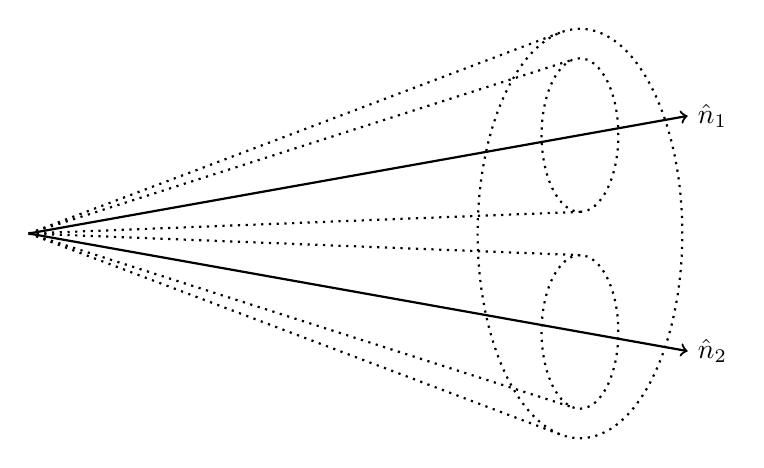
\begin{tikzpicture}
  % Main jet
  \draw[rotate around={270:(0,0)},dotted,thick] (0,7) ellipse (2.6 and 1.3);
  \draw[rotate around={270:(0,0)},dotted,thick] (0,0) -- (69.29:7.21);
  \draw[rotate around={270:(0,0)},dotted,thick] (0,0) -- (110.71:7.21);

  % Subjets
  \draw[rotate around={270:(0,0)},dotted,thick] (1.25,7) ellipse (0.975 and 0.4875);
  \draw[rotate around={270:(0,0)},dotted,thick] (0,0) -- (72.275:7.26);
  \draw[rotate around={270:(0,0)},dotted,thick] (0,0) -- (87.75:7.01);
  \draw[rotate around={270:(0,0)},dotted,thick] (-1.25,7) ellipse (0.975 and 0.4875);
  \draw[rotate around={270:(0,0)},dotted,thick] (0,0) -- (92.25:7.01);
  \draw[rotate around={270:(0,0)},dotted,thick] (0,0) -- (107.725:7.26);

  % Axes
  \draw[->,thick] (0,0) -- (10.12:8.5) node[right] {$\hat{n}_1$};
  \draw[->,thick] (0,0) -- (-10.12:8.5) node[right] {$\hat{n}_2$};
\end{tikzpicture}

  \caption{Illustration of jet substructure for a two-pronged jet with axes $\mathbf{\hat{n}}_1$ and $\mathbf{\hat{n}}_2$.}
  \label{fig:jet}
\end{figure}
